% ============================================================
%  fig03_timing_diagram.tex
%  Execution timing diagram for one RL trading environment step.
%  Causality-correct sequence diagram with explicit time axis.
%  Requires: tikz with libraries arrows.meta, positioning,
%            fit, backgrounds, calc
% ============================================================
\usetikzlibrary{arrows.meta,positioning,fit,backgrounds,calc}

% ------------------------------------------------------------------
%  Style definitions
% ------------------------------------------------------------------
\tikzset{
    actor/.style={
        draw=blue!55!black,
        fill=blue!12,
        rounded corners=3pt,
        minimum width=2.15cm,
        minimum height=9mm,
        align=center,
        font=\footnotesize\bfseries
    },
    lifeline/.style={
        dashed,
        draw=black!40,
        line width=0.5pt
    },
    event/.style={
        draw=green!50!black,
        fill=green!10,
        rounded corners=3pt,
        minimum width=2.10cm,
        minimum height=8mm,
        align=center,
        font=\footnotesize
    },
    arr/.style={
        -{Latex[length=2.2mm,width=1.6mm]},
        line width=0.85pt,
        draw=black!75
    },
    boundary/.style={
        draw=orange!75!black,
        dotted,
        line width=0.9pt
    },
    timeline/.style={
        -{Latex[length=2.4mm,width=1.7mm]},
        draw=black!70,
        line width=0.75pt
    },
    timetick/.style={
        draw=black!65,
        line width=0.55pt
    },
    msglabel/.style={
        font=\scriptsize,
        inner sep=1.2pt,
        fill=white,
        align=center
    },
    delaylabel/.style={
        font=\scriptsize\itshape,
        text=purple!65!black,
        fill=white,
        inner sep=1pt
    }
}

% ------------------------------------------------------------------
%  Diagram geometry
% ------------------------------------------------------------------
\newcommand{\COLSEP}{2.20cm}  % centre-to-centre actor spacing

\def\Yone{1.15}
\def\Ytwo{2.25}
\def\Ythree{3.35}
\def\Yfour{4.45}
\def\Yfive{5.55}
\def\Ysix{6.65}
\def\Yseven{7.75}
\def\Yeight{8.85}
\def\Ynine{9.95}
\def\Yten{11.05}
\def\YBOUND{5.00}
\def\LIFEBOT{11.85}

\begin{figure*}[!tbp]
\centering
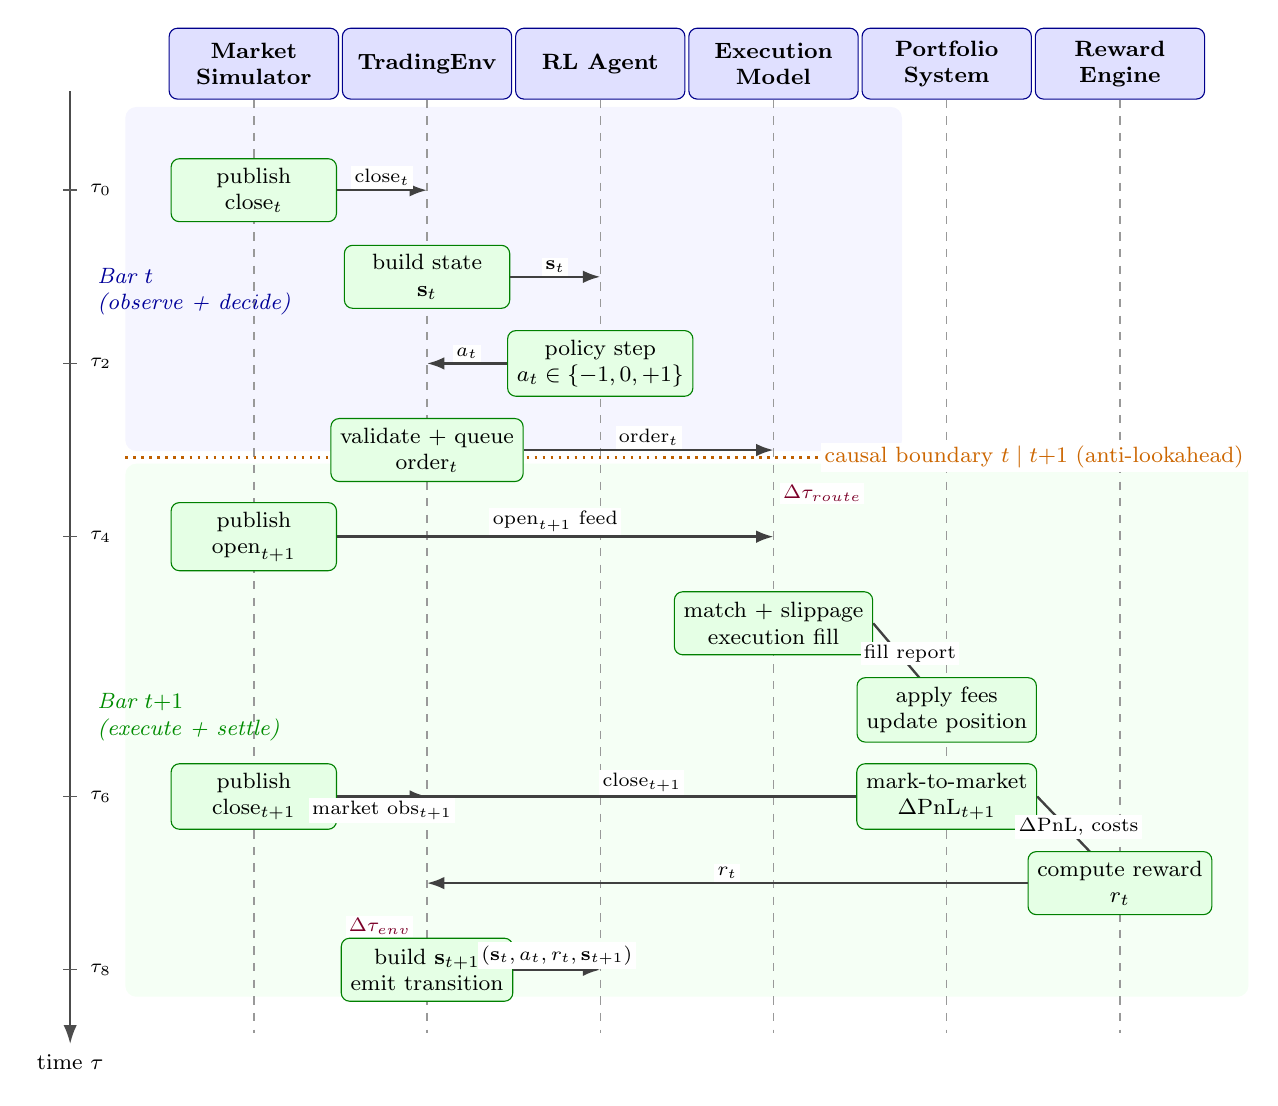
\begin{tikzpicture}[
    x=1cm,
    y=-1cm,
    node distance=0pt
]

% ==================================================================
% ACTOR HEADER ROW
% ==================================================================
\node[actor] (A_market)    at (0*\COLSEP,0) {Market\\Simulator};
\node[actor] (A_env)       at (1*\COLSEP,0) {TradingEnv};
\node[actor] (A_agent)     at (2*\COLSEP,0) {RL Agent};
\node[actor] (A_exec)      at (3*\COLSEP,0) {Execution\\Model};
\node[actor] (A_portfolio) at (4*\COLSEP,0) {Portfolio\\System};
\node[actor] (A_reward)    at (5*\COLSEP,0) {Reward\\Engine};

% ==================================================================
% LIFELINES
% ==================================================================
\foreach \actor in {A_market,A_env,A_agent,A_exec,A_portfolio,A_reward}{
    \draw[lifeline] (\actor.south) -- ($(\actor.south)+(0,\LIFEBOT)$);
}

% Coordinates on lifelines (structural timing grid)
\foreach \r/\y in {
    r1/\Yone,
    r2/\Ytwo,
    r3/\Ythree,
    r4/\Yfour,
    r5/\Yfive,
    r6/\Ysix,
    r7/\Yseven,
    r8/\Yeight,
    r9/\Ynine,
    r10/\Yten
}{
    \coordinate (mkt-\r) at ($(A_market.south)+(0,\y)$);
    \coordinate (env-\r) at ($(A_env.south)+(0,\y)$);
    \coordinate (agt-\r) at ($(A_agent.south)+(0,\y)$);
    \coordinate (exe-\r) at ($(A_exec.south)+(0,\y)$);
    \coordinate (pf-\r)  at ($(A_portfolio.south)+(0,\y)$);
    \coordinate (rew-\r) at ($(A_reward.south)+(0,\y)$);
}

% ==================================================================
% TIME AXIS + TICKS (explicit temporal reference)
% ==================================================================
\coordinate (TimeTop) at ($(A_market.west)+(-1.25cm,0.35)$);
\draw[timeline] (TimeTop) -- ($(TimeTop)+(0,\LIFEBOT+0.25)$)
    node[below,font=\footnotesize] {time $\tau$};

\coordinate (T1) at (TimeTop |- mkt-r1);
\coordinate (T2) at (TimeTop |- agt-r3);
\coordinate (T3) at (TimeTop |- mkt-r5);
\coordinate (T4) at (TimeTop |- mkt-r8);
\coordinate (T5) at (TimeTop |- env-r10);

\draw[timetick] ($(T1)+(-0.09,0)$) -- ($(T1)+(0.09,0)$);
\draw[timetick] ($(T2)+(-0.09,0)$) -- ($(T2)+(0.09,0)$);
\draw[timetick] ($(T3)+(-0.09,0)$) -- ($(T3)+(0.09,0)$);
\draw[timetick] ($(T4)+(-0.09,0)$) -- ($(T4)+(0.09,0)$);
\draw[timetick] ($(T5)+(-0.09,0)$) -- ($(T5)+(0.09,0)$);

\node[anchor=west,font=\scriptsize] at ($(T1)+(0.13,0)$) {$\tau_0$};
\node[anchor=west,font=\scriptsize] at ($(T2)+(0.13,0)$) {$\tau_2$};
\node[anchor=west,font=\scriptsize] at ($(T3)+(0.13,0)$) {$\tau_4$};
\node[anchor=west,font=\scriptsize] at ($(T4)+(0.13,0)$) {$\tau_6$};
\node[anchor=west,font=\scriptsize] at ($(T5)+(0.13,0)$) {$\tau_8$};

% ==================================================================
% CAUSAL BOUNDARY (horizontal: separates t from t+1 market info)
% ==================================================================
\draw[boundary]
    ($(A_market.west)+(-0.55cm,\YBOUND)$) -- ($(A_reward.east)+(0.55cm,\YBOUND)$)
    node[pos=1,above,anchor=east,font=\footnotesize,text=orange!80!black,fill=white,inner sep=1.3pt]
    {causal boundary $t\mid t{+}1$ (anti-lookahead)};

% ==================================================================
% EVENT FLOW (causality-correct MDP transition)
% ==================================================================
\node[event] (E_close_t) at (mkt-r1)
    {publish\\$\mathrm{close}_t$};
\draw[arr] (E_close_t.east) -- node[msglabel,above] {$\mathrm{close}_t$} (env-r1);

\node[event] (E_state_t) at (env-r2)
    {build state\\$\mathbf{s}_t$};
\draw[arr] (E_state_t.east) -- node[msglabel,above] {$\mathbf{s}_t$} (agt-r2);

\node[event] (E_action) at (agt-r3)
    {policy step\\$a_t\in\{-1,0,+1\}$};
\draw[arr] (E_action.west) -- node[msglabel,above] {$a_t$} (env-r3);

\node[event] (E_order) at (env-r4)
    {validate + queue\\order$_t$};
\draw[arr] (E_order.east) -- node[msglabel,above] {order$_t$} (exe-r4);

\node[delaylabel] at ($(exe-r4)!0.5!(exe-r5)+(0.62,0)$) {$\Delta\tau_{\text{route}}$};

\node[event] (E_open_tp1) at (mkt-r5)
    {publish\\$\mathrm{open}_{t+1}$};
\draw[arr] (E_open_tp1.east) -- node[msglabel,above] {$\mathrm{open}_{t+1}$ feed} (exe-r5);

\node[event] (E_fill) at (exe-r6)
    {match + slippage\\execution fill};
\draw[arr] (E_fill.east) -- node[msglabel,above] {fill report} (pf-r7);

\node[event] (E_portfolio) at (pf-r7)
    {apply fees\\update position};

\node[event] (E_close_tp1) at (mkt-r8)
    {publish\\$\mathrm{close}_{t+1}$};
\draw[arr] (E_close_tp1.east) -- node[msglabel,above] {$\mathrm{close}_{t+1}$} (pf-r8);
\draw[arr] (E_close_tp1.east) -- node[msglabel,below] {market obs$_{t+1}$} (env-r8);

\node[event] (E_mark) at (pf-r8)
    {mark-to-market\\$\Delta\mathrm{PnL}_{t+1}$};
\draw[arr] (E_mark.east) -- node[msglabel,above] {$\Delta\mathrm{PnL}$, costs} (rew-r9);

\node[event] (E_reward) at (rew-r9)
    {compute reward\\$r_t$};
\draw[arr] (E_reward.west) -- node[msglabel,above] {$r_t$} (env-r9);

\node[delaylabel] at ($(env-r9)!0.5!(env-r10)+(-0.60,0)$) {$\Delta\tau_{\text{env}}$};

\node[event] (E_transition) at (env-r10)
    {build $\mathbf{s}_{t+1}$\\emit transition};
\draw[arr] (E_transition.east)
    -- node[msglabel,above] {$(\mathbf{s}_t,a_t,r_t,\mathbf{s}_{t+1})$}
    (agt-r10);

% ==================================================================
% BACKGROUND PHASE SHADING
% ==================================================================
\begin{scope}[on background layer]
    \fill[blue!4,rounded corners=4pt]
        ($(A_market.west)+(-0.55cm,0.55)$)
        rectangle
        ($(A_exec.east)+(0.55cm,4.92)$);

    \fill[green!4,rounded corners=4pt]
        ($(A_market.west)+(-0.55cm,5.08)$)
        rectangle
        ($(A_reward.east)+(0.55cm,\LIFEBOT)$);
\end{scope}

\node[
    font=\footnotesize\itshape,
    text=blue!60!black,
    align=left,
    anchor=west
] at ($(TimeTop)+(0.22,2.55)$) {Bar $t$\\(observe + decide)};

\node[
    font=\footnotesize\itshape,
    text=green!55!black,
    align=left,
    anchor=west
] at ($(TimeTop)+(0.22,7.95)$) {Bar $t{+}1$\\(execute + settle)};

\end{tikzpicture}

\caption{Causality-correct environment step timing: the environment emits $\mathbf{s}_t$, receives $a_t$, execution is driven by market $\mathrm{open}_{t+1}$, portfolio state is marked at $\mathrm{close}_{t+1}$, reward engine returns only $r_t$ to the environment, and the environment emits the full transition $(\mathbf{s}_t,a_t,r_t,\mathbf{s}_{t+1})$ without any Reward$\rightarrow$Agent bypass.}
\label{fig:timing_diagram}
\end{figure*}